\chapter{Metodologia} \label{label_revisao_bib}
\section{Eletroencefalograma (EEG)}
\subsection{Caracter\'isticas e Sistemas de Medi\c{c}\~ao}
\par
O \ac{EEG} \'e uma das t\'ecnicas n\~ao invasivas mais populares para o desenvolvimento de \ac{BCIs} devido \`a sua alta resolu\c{c}\~ao temporal, baixo custo e por ser de f\'acil instala\c{c}\~ao \cite{RAO}.
\par
Sinais \ac{EEG}, coletados da superf\'icie do couro cabeludo s\~ao flutua\c{c}\~oes de pot\^enciais el\'etricos que refletem a atividade no c\'erebro  principalmente no c\'ortex cerebral abaixo da superf\'cie do couro cabeludo \cite{Vidal77}.
%\par
%O \ac{EEG} consiste em posicionar eletrodos no couro cabeludo.
%Sinais de \ac{EEG} refletem  o somat\'orio de potenciais p\'os-sin\'apticos de milhares de neur\^onios orientados radialmente ao couro cabeludo.
Correntes origin\'arias de regi\~oes mais profundas n\~ao s\~ao detectadas devido ao fato de que campos el\'etricos decaem com o quadrado da dist\^ancia de sua origem.
Portanto, o \ac{EEG} predominantemente captura a atividade no c\'ortex cerebral, cujo o arranjo colunar de neur\^onios e proximidade ao cr\^anio favorecem a sua captura \cite{RAO}.
\par
O padrão internacional sistema 10-20 é tipicamente utilizado para a gravação de \ac{EEG}. Nesse sistema 21 eletrodos são posicionados na superfície do couro cabeludo.
O posicionamento é determinado da seguinte maneira: Os pontos de referência são o n\'asion, que está localizado acima do nariz no nível dos olhos e o ínion que é o ressalto ossudo na base da cr\^anio na linha central do traseiro da cabeça. A partir desses pontos, o perímetro da c é medido dividindo nos planos transverso e mediano. Os locais dos eletrodos podem ser determinadas dividindo esses perímetros em intervalos de 10\% e 20\%. Três outros eletrodos são posicionados em ambos os lados equidistantes dos pontos vizinhos como mostrado na figura \ref{fig:10-20}. \cite{EEGPrinciple}
\begin{figure}[!ht]
	\begin{center}
		\caption{Posi\c{c}\~oes do sistema 10-20 sobre um cr\^anio. Obtido em \cite{EEGPrinciple} }		
		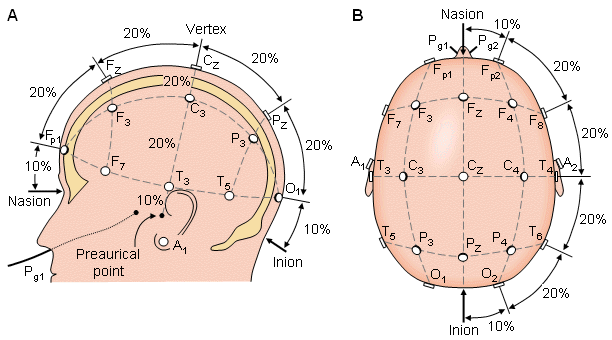
\includegraphics[scale=1]{./figuras/10-20_cranio}
		\label{fig:10-20}
	\end{center}
\end{figure}
\par
Eletrodos bipolares e monopolares podem ser utilizados para a medição do \ac{EEG} (fig. \ref{fig:bipolar-vs-monopolar}).
 No primeiro método é medido a diferença entre um par de eletrodos (fig. \ref{fig:bipolar-vs-monopolar}-A).
 No método posterior o potencial de cada eletrodo é comparado a um eletrodo neutro ou \`a m\'edia de todos os eletrodos como pode ser observado na figura \ref{fig:bipolar-vs-monopolar}-B \cite{EEGPrinciple}.
\begin{figure}[!ht]
	\begin{center}
		\caption{Compara\c{c}\~ao do sinal Monopolar (B) vs o Bipolar (A). Obtido em \cite{EEGPrinciple} }		
		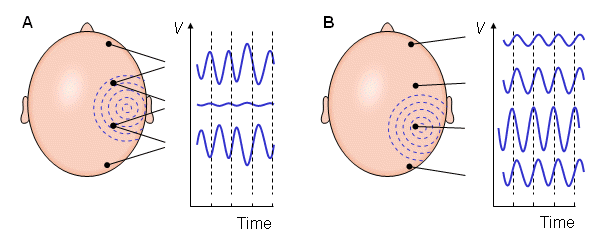
\includegraphics[scale=1]{./figuras/Bipolar-vs-Monopolar}
		\label{fig:bipolar-vs-monopolar}
	\end{center}
\end{figure}
\clearpage
\subsection{Ritmo $\mu$}
No \ac{EEG}, em humanos a regi\~ao pr\'oxima ao c\'ortex motor exibe tipicamente um sinal, de 10$\mu V$-50$\mu V$ e na banda de frequ\^encia de aproximadamente 8-12Hz, enquanto n\~ao est\'a produzindo atividade motora, este sinal \'e denominado de ritmo  $\mu$ (figura \ref{fig:Mu}).
Movimento real ou imagin\'ario \'e normalmente acompanhada de uma redu\c{c}\~ao no ritmo $\mu$ no lado do c\'erebro oposto ao movimento como pode ser visto na figura \ref{fig:mu-left-vs-right}.
Est\'a redu\c{c}\~ao de atividade \'e referida como \ac{ERD} por \cite{EOG2006} e como \ac{ERS} por \cite{Vidal77}.
\cite{BCI2000} \cite{RAO}
\begin{figure}[!ht]
	\begin{center}
		\caption{(A,B) distribui\c{c}\~ao topogr\'afica no couro cabeludo da diferen\c{c}a calculada do movimento da m\~ao direita (A) real e (B) imagin\'ario de uma pessoa vs ela relaxada com o sinal numa banda 10,5-13,5Hz. (C) O espectro  para um outro sujeito em C3 comparando o estado relaxado (linha cortada) vs imagina\c{c}\~ao motora e (D) o espectro $r^2$ para a imagina\c{c}\~ao motora vs o estado relaxado deste sujeito \cite{BCI2000}}
		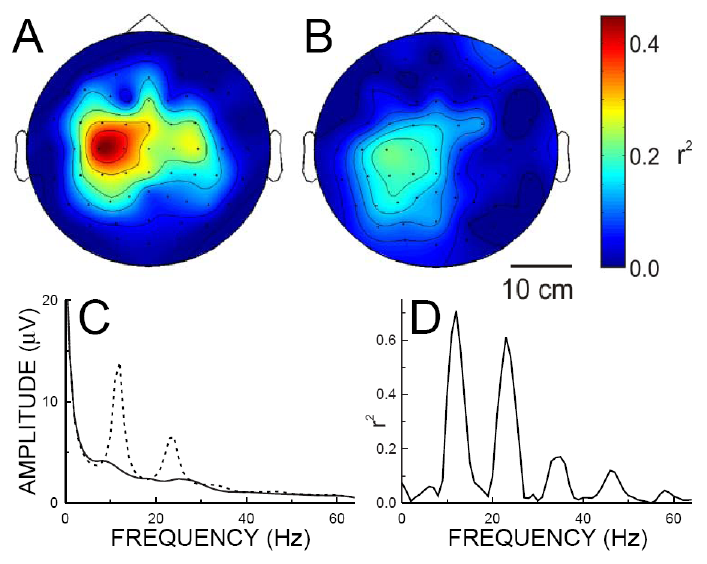
\includegraphics[scale=0.35]{./figuras/ERDmu}
		\label{fig:Mu}
	\end{center}
\end{figure}
\begin{figure}[!ht]
	\begin{center}
		\caption{O Efeito da imagina\c{c}\~ao motora esquerda vs direita no ritimo $\mu$ tal como captado pelos eletrodos em C3 (lado esquerdo) e C4 (lado direito) \cite{Qin2004}} 		
		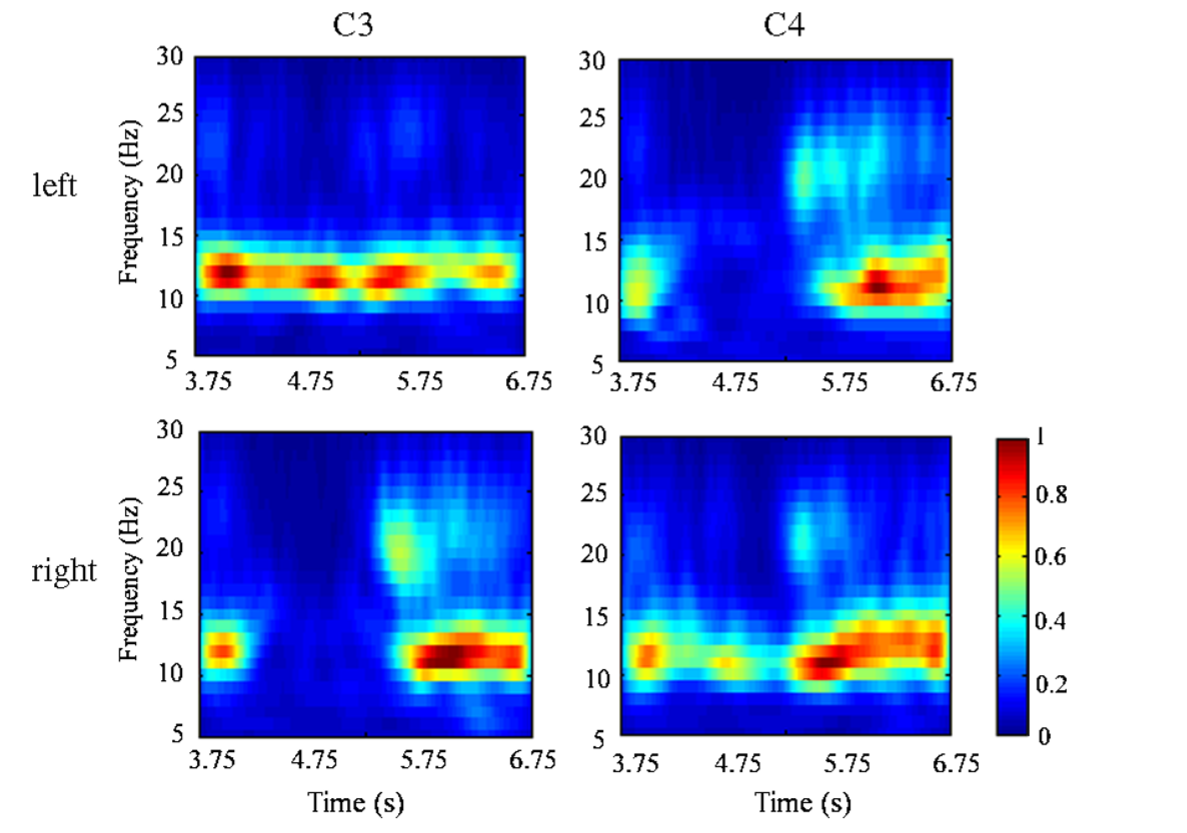
\includegraphics[scale=0.45]{./figuras/mu-left-vs-right}
		\label{fig:mu-left-vs-right}
	\end{center}
\end{figure}
\subsection{Redu\c{c}\~ao de Artefatos}
\par
Artefatos s\~ao flutua\c{c}\~oes pot\^encias de origem n\~ao neural. Essas incluem pot\^encias eletro oculares, musculares (do pesco\c{c}o, couro cabeludo e do rosto), \ac{ECG} al\'em de fontes externas como o ru\'ido de rede el\'etrica 50/60Hz  \cite{Vidal77} \cite{RAO}.
\par
Artefatos no geral e especificamente no \ac{EOG} s\~ao uma grande fonte de ru\'idos em grava\c{c}\~oes de \ac{EEGs}.
Pode-se assumir que toda grava\c{c}\~ao \ac{EEG} est\'a contaminada com artefatos \ac{EOG}, pois movimentos oculares s\~ao dif\'iceis de suprimir por per\'iodos prolongados.
Por exemplo um estudo em \ac{EEG} do sono 9.1\% do total grava\c{c}\~ao estava contaminada com artefatos \ac{EOG} \cite{EOG2006}.
\par
A origem do \ac{EOG} \'e devido \`a atividade el\'etrica do olho que \'e propagada pelo corpo e pode ser gravado pelo corpo em sua superf\'icie.
Artefatos \ac{EOG} s\~ao causados pelos movimentos do dipolo retinal e das p\'alpebras.
Um modelo simplificado assume um dipolo el\'etrico dentro dos olhos.
A dire\c{c}\~ao do dipolo \'e alinhada com a linha de vis\~ao e a amplitude do dipolo \'e determinada pela quantidade de luz atingindo a retina.
Na maioria dos casos ambos olhos est\~ao na mesma linha de vis\~ao e observam a mesma lumin\^ancia. Portanto ambos os dipolos s\~ao paralelos e altamente correlacionados.
Por conta disso o \ac{EOG} pode ser modelado por um \'unico dipolo. 
Devido aos efeitos da condu\c{c}\~ao de volume, o \ac{EOG} e \ac{EEG} s\~ao propagados pela superf\'icie da cabe\c{c}a onde a superposi\c{c}\~ao de ambos \'e gravado.
Os pesos dos componentes dessas superposi\c{c}\~ao s\~ao determinados pelas rela\c{c}\~oes espaciais e propriedades el\'etricas dos tecidos entre as fontes e os eletrodos.
Essas propriedades n\~ao se alteram durante uma grava\c{c}\~ao com a exce\c{c}\~ao do movimento das p\'alpebras que alteram a geometria do tecido proximo delas.
Por\'em esse efeito do movimento das p\'alpebras pode ser modelado como uma componente radial do \ac{EOG}, portanto os pesos dos componentes na superposi\c{c}\~ao podem ser considerados est\'aticos \cite{EOG2006}.
\par
Para a redu\c{c}\~ao de artefatos \ac{EOG} existem v\'arias t\'ecnicas dentre elas \ac{PCA}, \ac{ICA} e regress\~ao linear.
A seguir ser\'a descrito o m\'etodo discutido em \cite{EOG2006} que \'e uma regress\~ao linear.
\par
O seguinte modelo linear \'e assumido contendo 3 componentes espaciais (horizontal, vertical e radial) de \ac{EOG}: 
\begin{equation}
Y(t,ch)=S(t,ch)+[EOG1(t),EOG2(t),EOG3(t)]
\cdotp
[b_1(ch),b_2(ch),b_3(ch)]^T
\end{equation}
Onde $Y(t,ch)$ \'e o valor gravado de cada canal ch num tempo t, S \'e a fonte do sinal sem contami\c{c}\~ao de artefatos, EOG123 indicam a fonte de ruido $U$ das 3 componentes espaciais do EOG e $b(ch)$ indicam os pesos dos componentes EOG no canal \ac{EEG} ch.
Para podermos obter o sinal corrigido a fonte de ru\'idos $U$ e os pesos $b$ tem que serem conhecidos.
O \ac{EOG} pode ser gravado num canal separado.
Para obter $b$  tem que se assumir de que o sinal $S$ e o ru\'ido $U$ s\~ao linearmente independentes, assumindo isso.
\begin{equation}
S=Y-U \cdotp b
\end{equation}
\begin{equation}
<U^T S>=<U^T Y> - <U^T U>b
\end{equation}
onde $<U^T S>=0$ resultando em
\begin{equation}
b=<U^T U>^{-1} <U^T Y>
\end{equation}
permitindo que $S$ seja calculado.
\clearpage
\section{Redes Neurais}
\par
Redes neurais baseadas em Backpropagation tem se mostrado bem sucedido em uma alta variedade de tarefas de classifica\c{c}\~ao , incluindo a classifica\c{c}\~ao de dados de \ac{BCI}.
Apesar de serem poderosas tais redes neurais frequentemente sofrem de um problema de \textit{overfitting} aos dados de treinamento, resultando numa genereliza\c{c}\~ao fraca.
Por consequ\^encia disso \ac{SVM}s s\~ao tipicamente favorecidas sobre \ac{ANN} como o algor\'itmo de escolha em muitas \ac{BCI} \cite{RAO}. Mas o seu entendimento ainda \'e importante, pois novas t\'ecnicas est\~ao sendo derivadas de \ac{ANN} tal como Redes Neurais Convolucionais \cite{nigam2020}. 
\par
\ac{ANN} s\~ao inspiradas pela sua contraparte na biologia e procuram reproduzir algumas das capacidades adaptativas de redes neurais no c\'erebro em classificar dados de entrada de maneira robusta \cite{Haykin2008}. 

\subsection{Neur\^onios Artificiais}
O modelo de um neur\^onio que forma as \ac{ANN} \'e mostrado na figura \ref{fig:neuronioartificial} e consiste em 3 partes:
\begin{enumerate}
	\item Um conjunto de sin\'apses (conex\~oes) cada uma caracterizada por um peso $w_{l\left< k,j \right> }$ onde $k$ \'e o \'indice do neur\^onio na camada $l$ e $j$ \'e o \'indice do n\'o de origem na camada anterior ($l-1$).
	\item Um somador para somar todos os sinais de entrada multiplicado pelo seu \textbf{peso} $w_{l\left< k,j \right> }$ e o valor do \textbf{bias} $b_{(l,k)}$.
	\item Uma fun\c{c}\~ao de ativa\c{c}\~ao $\varphi(s)$ para restringir a amplitude da sa\'ida de um neur\^onio. tipicamente a amplitude da saida de um neur\^onio varia de [0,1] ou [-1,1].
\end{enumerate}
Este modelo tamb\'em pode ser representado por esse par de equa\c{c}\~oes:
\begin{equation}
s=\sum_{j=1}^{n} w_{l\left< k,j \right> } x_j
\end{equation}
e
\begin{equation}
y_k=\varphi \left( s+b_{(l,k)} \right) 
\end{equation}
\begin{figure}[!h]
	\begin{center}
		\caption{Diagrama neuronio}		
		\tikzstyle{weightNode}=[draw,rectangle,minimum size=10pt,inner sep=3pt]
\tikzstyle{stateTransition}=[->, thick]
\tikzstyle{biasNode}=[-stealth]
\tikzstyle{nonlinearityNode}=[draw,rectangle,minimum size=25pt, inner sep=2pt]
\begin{tikzpicture}
\node[draw,circle,minimum size=25pt,inner sep=0pt] (x) at (0,0) {$\Sigma$};
\foreach \l [count=\n] in {0,1,2,3,n} {
	\node[weightNode] (w\l) at (-2.2,{1.1*(3-(\n))}) {$ w_{l \left< k ,\l \right>}$};
	\draw[stateTransition] (w\l) to [out=0,in={82.5+\n*32.5}] node [midway, sloped, above=-2] {} (x);
	\node[biasNode] (x\l) at (-3.7,{1.1*(3-(\n))}){$x_\l$};
	\draw[stateTransition,o->] (x\l) -- (w\l);
}
\node[biasNode]  (b)  at (0,2) {$b_{(l,k)}$};
\node[nonlinearityNode] (phi) at (1.75,0) {$\varphi \small{\left(  s \right)  } $};
\draw[stateTransition] (phi) -- (3,0) node [midway,above=-0.1cm] {$y_k$};
\draw[stateTransition,o->] (b) -- (x);
\draw[stateTransition] (x) -- (phi);
\node (dots) at (-3.75, -1.5) {$\vdots$};
\end{tikzpicture}
		\label{fig:neuronioartificial}
	\end{center}	
\end{figure}
\subsection{Tipos de Fun\c{c}\~oes de ativa\c{c}\~ao}
\begin{itemize}
	\item \textbf{Fun\c{c}\~ao Sinal}: \'e uma fun\c{c}\~ao de ativa\c{c}\`ao simples descrita pela equa\c{c}\~ao \ref{eq:sign}.
	\begin{equation}\label{eq:sign}
	\varphi \left( s \right) =\begin{cases}
	1 \text{ se } s > 0\\
	0 \text{ se } s = 0\\
	-1 \text{ se } s < 0
	\end{cases}
	\end{equation}
	Ela \'e uma das fun\c{c}~oes de ativa\c{c}\~ao mais simples e \'e utilizada no perceptron de uma camada, \ac{LDA} e \ac{SVM} entre outros.
	\begin{figure}[!h]
		\begin{center}
			\caption{Fun\c{c}\~ao Sinal}			
			\begin{tikzpicture}[domain=-1.5:1.5,scale=2]
%\draw[very thin,color=gray,step=0.25] (-1.4,-1.4) grid (1.4,1.4);
\draw[loosely dashed,thick](-1.6,-1) -- (+1.6,-1) node[right] {$-1$};
\draw[loosely dashed,thick](-1.6,1) -- (+1.6,1) node[right] {$1$};
\draw[->] (-1.6,0) -- (1.6,0) node[right]{$s$};
\draw[->] (0,-1.6) -- (0,1.6) node[above]{$\varphi \left( s \right) $};
\draw[color=cyan,very thick] (-1.6,-1) -- (-0.015,-1);
\draw[dotted,color=cyan,very thick] (-0.015,-1) -- (0.015,1);
\draw[color=cyan,very thick] (0.015,1) -- (1.6,1);
\end{tikzpicture}
			\label{fig:funcaosinal}
		\end{center}	
	\end{figure}
	\item \textbf{Fun\c{c}\~ao Logi\'stica}
	\'e uma fun\c{c}\~ao do tipo sigm\'oide, cujo gr\'afico tem forma de s, \'e a fun\c{c}\~ao de ativa\c{c}\~ao mais comum para o uso em \ac{ANN}. Ela tem uma amplitude de [0,1] ela \'e dada pela equa\c{c}\~ao \ref{eq:log}.
	\begin{equation}\label{eq:log}
	\varphi \left( s \right) = \frac{1}{1+exp(-a s)}
	\end{equation}
	Ela \'e deriv\'avel e sua derivada \'e extremamente simples e dada por eq. \ref{eq:divlog}
	\begin{equation}\label{eq:divlog} 
	\dv{\varphi \left( s \right)}{s}  = \varphi \left( s \right)\left( 1 -  \varphi \left( s \right) \right)
	\end{equation}	
	\begin{figure}[!ht]
		\begin{center}
			\caption{Fun\c{c}\~ao log\'istica}			
			\begin{tikzpicture}[domain=-1.5:1.5,scale=2]
%\draw[very thin,color=gray,step=0.25] (-1.4,-1.4) grid (1.4,1.4);
\draw[loosely dashed,thick](-1.6,-1) -- (+1.6,-1) node[right] {$-1$};
\draw[loosely dashed,thick](-1.6,1) -- (+1.6,1) node[right] {$1$};
\draw[->] (-1.6,0) -- (1.6,0) node[right]{$s$};
\draw[->] (0,-1.6) -- (0,1.6) node[above]{$\varphi \left( s \right) $};
\draw[very thick,color=cyan] plot (\x,{1/(1+exp(-5*\x))});
\end{tikzpicture}
			\label{fig:funcaologistica}
		\end{center}	
	\end{figure}
	\item \textbf{Fun\c{c}\~ao tangente hiperb\'olica} \'e uma outra fun\c{c}\~ao do tipo sigm\'oide sua amplitude \'e de [-1,1] o fato de ser uma fun\c{c}\~ao impar reduz o numero de itera\c{c}\~oes nescess\'arias se comparado \`a fun\c{c}\~ao log\'istica (mais detalhes sobre isso pode-se encontrar em \cite{Haykin2008} se\c{c}\~ao 4.11). 
	\begin{equation} \label{eq:tanh}
	\varphi \left( s \right)  = tanh(s)
	\end{equation}	
	E sua derivada Eq. \ref{eq:divtanh}.
	\begin{equation}\label{eq:divtanh}
	\dv{\varphi \left( s \right)}{s}  = 1 -  \varphi^2 \left( s \right) 
	\end{equation}	
	\begin{figure}[!h]
		\begin{center}
			\caption{Fun\c{c}\~ao tangente hiperb\'olica}			
			\begin{tikzpicture}[domain=-1.5:1.5,scale=2]
%\draw[very thin,color=gray,step=0.25] (-1.4,-1.4) grid (1.4,1.4);
\draw[loosely dashed,thick](-1.6,-1) -- (+1.6,-1) node[right] {$-1$};
\draw[loosely dashed,thick](-1.6,1) -- (+1.6,1) node[right] {$1$};
\draw[->] (-1.6,0) -- (1.6,0) node[right]{$s$};
\draw[->] (0,-1.6) -- (0,1.6) node[above]{$\varphi \left( s \right) $};
\draw[very thick,color=cyan] plot (\x,{tanh(2*\x)});
\end{tikzpicture}
			\label{fig:funcaotanh}
		\end{center}	
	\end{figure}	
\end{itemize}
\subsection{Perceptron de m\'ultiplas camadas}
\par
As \ac{ANN} chamadas de \ac{MLP} consistem tipicamente de um conjunto de n\'os de entrada que constituem a \textit{camada de entrada}, uma ou mais \textit{camadas ocultas} e uma \textit{camada de sa\'ida} isto pode ser visto na figura \ref{fig:MLP} \cite{Haykin2008}.

\begin{figure}[!h]
	\begin{center}
		\caption{Diagrama de MLP gen\'erico}		
		\tikzset{%
  every neuron/.style={
    circle,
    draw,
    minimum size=1cm
  },
  neuron missing/.style={
    draw=none, 
    scale=2,
    text height=0.333cm,
    execute at begin node=\color{black}$\vdots$
  },
  every input/.style={
  	rectangle,
  	draw,
  	minimum size=0.2cm
  },
  input missing/.style={
	draw=none, 
	scale=2,
	text height=0.333cm,
	execute at begin node=\color{black}$\vdots$
},
}

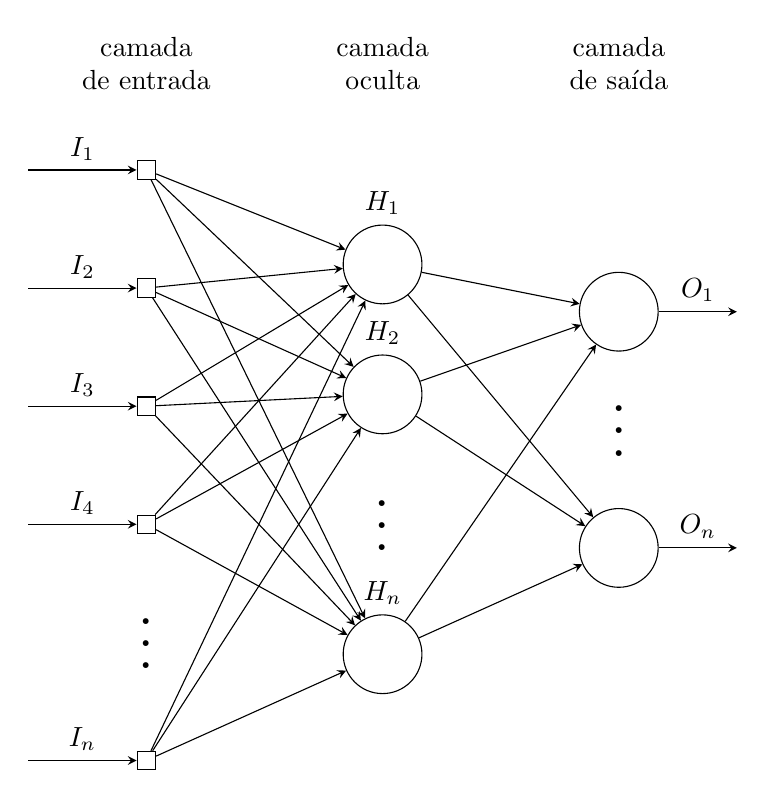
\begin{tikzpicture}[x=1.5cm, y=1.5cm, >=stealth]

\foreach \m/\l [count=\y] in {1,2,3,4,missing,5}
  \node [every input/.try, input \m/.try] (input-\m) at (0,2.7-\y) {};

\foreach \m [count=\y] in {1,2,missing,3}
  \node [every neuron/.try, neuron \m/.try ] (hidden-\m) at (2,2-\y*1.1) {};

\foreach \m [count=\y] in {1,missing,2}
  \node [every neuron/.try, neuron \m/.try ] (output-\m) at (4,1.5-\y) {};

\foreach \l [count=\i] in {1,2,3,4,n}
  \draw [<-] (input-\i) -- ++(-1,0)
    node [above, midway] {$I_\l$};

\foreach \l [count=\i] in {1,2,n}
  \node [above] at (hidden-\i.north) {$H_\l$};

\foreach \l [count=\i] in {1,n}
  \draw [->] (output-\i) -- ++(1,0)
    node [above, midway] {$O_\l$};

\foreach \i in {1,...,5}
  \foreach \j in {1,...,3}
    \draw [->] (input-\i) -- (hidden-\j);

\foreach \i in {1,...,3}
  \foreach \j in {1,...,2}
    \draw [->] (hidden-\i) -- (output-\j);

\foreach \l [count=\x from 0] in {de entrada, oculta, de sa\'ida}
  \node [align=center, above] at (\x*2,2.3) {camada \\ \l};

\end{tikzpicture}
		\label{fig:MLP}
	\end{center}	
\end{figure}
\par
Um \ac{MLP} tem tr\^es caracter\'isticas distintivas \cite{Haykin2008}:
\begin{enumerate}
	\item 	O modelo de cada neur\^onio inclui uma fun\c{c}\~ao de ativa\c{c}\~ao n\~ao-linear continuamente diferenci\'avel.
	A n\~ao linearidade \'e nescess\'aria pois sem ela a rede pode ser reduzida a uma \'unica camada (a camada de sa\'ida).
	\item  A rede cont\'em uma ou mais camadas de neur\^onios ocultos, que n\~ao fazem parte da entrada ou sa\'ida da rede. 
	\item A rede exibe um alto grau de \textbf{conectividade}, determinado pelas sinapses da rede.
\end{enumerate}
\subsection{Aprendizagem}
Dentre das regras de aprendizagem uma das mais antigas \'e a aprendizagem Hebbiana que simplificada diz \cite{Haykin2008}:
\begin{enumerate}
	\item Quando dois neur\^onios em ambos os lados da sinapse s\~ao ativados ao mesmo tempo o peso da conex\~ao entre eles \'e fortalecido.
	\item Quando dois neur\^onios em ambos lados da sinapse s\~ao ativados de maneira dessincronizada o peso da conex\~ao entre eles \'e enfraquecido.
\end{enumerate}
No caso do \acl{MLP} isto pode ser descrito pela eq. \ref{eq:Hebb} onde $\textbf{w}_n$ \'e o vetor dos pesos e bias da rede na itera\c{c}\~ao $n$.  
\begin{eqnarray}\label{eq:Hebb}
\textbf{w}_{n+1}=\textbf{w}_n+\Delta \textbf{w}_n\\
\textbf{w}=\left(w_{1\left< 1,1 \right> },\dots,w_{1\left< 1,j \right>},b_{\left(1,1 \right)},\dots,w_{L\left< K,J \right>},b_{\left(L,K \right)} \right)
\end{eqnarray}
Para determinar o valor de $\Delta \textbf{w}_n$, uma abordagem \'e escolher um  $\Delta \textbf{w}_n$ que minimize o erro de classifica\c{c}\~ao da rede num conjunto de treinamento. Essa abordagem \'e denominada \textit{aprendizagem por corre\c{c}\~ao de erro} \cite{Haykin2008} e pode ser formulada pela eq. \ref{eq:AprendizagemErro} onde, $\eta$ \'e o tamanho do passo, tamb\'em conhecido como \textit{taxa de aprendizagem}  e $\textbf{p}_n$ \'e um vetor com a dire\c{c}\~ao que minimiza a fun\c{c}\~ao de erro  de clasifica\c{c}\~ao $E(\textbf{w})$.
\begin{equation}\label{eq:AprendizagemErro}
\Delta \textbf{w}_n= \eta \textbf{p}_n
\end{equation}

\subsection{Backpropagation(BP)}

O algoritmo Backpropagation é um algoritmo que lida com os pesos de uma rede de acordo com os erros obtidos em seus neurônios adjacentes.  Ele utiliza um método gradiente como tentativa de minimizar o erro $E_{total}(\textbf{t},\textbf{o})$ entre os valores de saída e os valores alvos. A equação \ref{eq:backpropagation} mostra o principio básico do calculo para o erro, sendo a métrica utilizada em algoritmos b\'asicos o MSE (Erro médio quadrático). Sendo N o número de amostras, $t_n$ é a reposta alvo e $o_n$ é a resposta calculada da rede \cite{Haykin2008}.


\begin{equation}\label{eq:backpropagation}
E_{total}(\textbf{t},\textbf{o})  = \frac{1}{2N} \sum_{n=0}^{N} (t_n - o_n)^2
\end{equation}

Para cada entrada $I_{1}$ e $I_{2}$ e saída $O_{1}$ da Figura \ref{fig:BPNN} teremos:
\begin{itemize}
	\item A propagação das entradas $I_{1}$ e $I_{2}$ pela rede, e computando a saída $O_{1}$ para cada dado de treinamento.
	\item Para a saída $O_{1}$ é calculado então um erro $E_{total}(\textbf{t},\textbf{o})$ que está relacionado \`a sua sa\'ida e o resultado alvo esperado.
	\item A partir disso é calculado os erros dos pesos, utilizando a regra da cadeia, aos neurônios ocultos das camadas internas. Retropropagando o erro desde as camadas de saída até a ultima camada interna (figura \ref{fig:BPNNAmp}).
	\item Após o calculo dos erros de cada neur\^onio, é utilizado um método gradiente para o cálculo das novas sinapses de cada conexão. A equação \ref{eq:bpgradi} mostra um modo de como pode ser atualizado o peso sendo $\Delta w_{ij}$ o peso da conexão entre os neurônios i e j, $\eta$ a Taxa de aprendizado e $E_(w)$ o próprio erro. 
\end{itemize}
\par
Para classifica\c{c}\~ao uma das fun\c{c}\~oes de erro mais utilizadas \'e entropia cruzada.
Ela penaliza fortemente classifica\c{c}\~oes incorretas e \'e dada pela eq. \ref{eq:crossentropy} onde $o_n$ \'e a sa\'ida $n$ da rede e $t_n$ \'e o valor alvo daquela sa\'ida.
\begin{eqnarray}\label{eq:crossentropy}
E_n(t_n,o_n) = \frac{-t_n log(o_n)}{N}\\
E_{total}(\textbf{t},\textbf{o}) = \sum_{n=0}^{N} \frac{-t_n log(o_n)}{N}
\end{eqnarray}
e sua derivada \'e
\begin{equation}\label{eq:divcrossentropy}
\dv{E_n(t_n,o_n)}{o_n} = \frac{-t_n}{o_n N}\\
\end{equation}
\begin{equation}\label{eq:bpgradi}
\Delta w_{ij} = -\eta \frac{\partial E_(w) }{\partial w_{ij}}
\end{equation}


\begin{figure}[!htp]
	\begin{center}
		\caption{Exemplo de NN para calcular o Backpropagation}		
		\tikzset{%
  every neuron/.style={
    circle,
    draw,
    minimum size=1cm
  },
  neuron missing/.style={
    draw=none, 
    scale=2,
    text height=0.333cm,
    execute at begin node=\color{black}$\vdots$
  },
  every input/.style={
  	rectangle,
  	draw,
  	minimum size=0.2cm
  },
  input missing/.style={
	draw=none, 
	scale=2,
	text height=0.333cm,
	execute at begin node=\color{black}$\vdots$
},
}

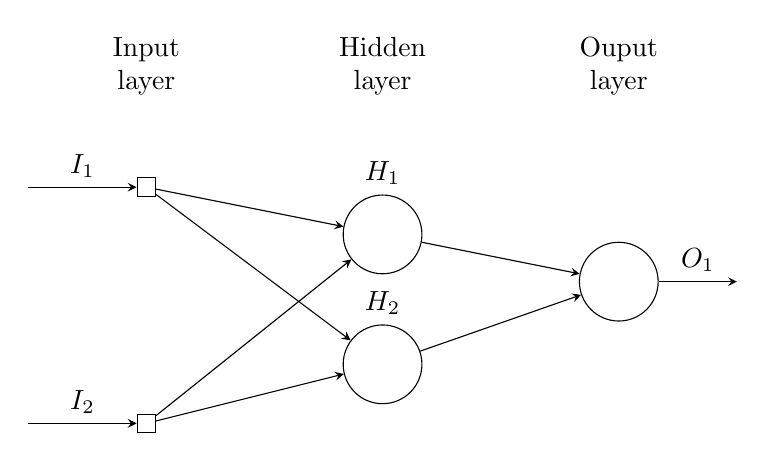
\begin{tikzpicture}[x=1.5cm, y=1.5cm, >=stealth]

\foreach \m/\l [count=\y] in {1,2}
  \node [every input/.try, input \m/.try] (input-\m) at (0,{1.3-(\y-1)*2}) {};

\foreach \m [count=\y] in {1,2}
  \node [every neuron/.try, neuron \m/.try ] (hidden-\m) at (2,2-\y*1.1) {};

\foreach \m [count=\y] in {1}
  \node [every neuron/.try, neuron \m/.try ] (output-\m) at (4,1.5-\y) {};

\foreach \l [count=\i] in {1,2}
  \draw [<-] (input-\i) -- ++(-1,0)
    node [above, midway] {$I_\l$};

\foreach \l [count=\i] in {1,2}
  \node [above] at (hidden-\i.north) {$H_\l$};

\foreach \l [count=\i] in {1}
  \draw [->] (output-\i) -- ++(1,0)
    node [above, midway] {$O_\l$};

\foreach \i in {1,...,2}
  \foreach \j in {1,...,2}
    \draw [->] (input-\i) -- (hidden-\j);

\foreach \i in {1,...,2}
  \foreach \j in {1}
    \draw [->] (hidden-\i) -- (output-\j);

\foreach \l [count=\x from 0] in {Input, Hidden, Ouput}
  \node [align=center, above] at (\x*2,2) {\l \\ layer};

\end{tikzpicture}
		\label{fig:BPNN}
	\end{center}	
\end{figure}
\begin{figure}[!htp]
	\begin{center}
		\caption{NN amp}		
		\tikzstyle{weightNode}=[draw,rectangle,minimum size=10pt,inner sep=3pt]
\tikzset{%
   input/.style={
	rectangle,
	draw,
	minimum size=0.2cm
},
}
\tikzstyle{stateTransition}=[->, thick]
\tikzstyle{biasNode}=[-stealth]
\tikzstyle{nonlinearityNode}=[draw,rectangle,minimum size=25pt, inner sep=2pt]
\begin{tikzpicture}

\node[draw,circle,minimum size=25pt,inner sep=0pt] (x3) at (0,0) {$\Sigma$};
\foreach \l [count=\n] in {1,2} {
	\node[weightNode] (w3\l) at (-2, {1-((\n-1)*2)}) {$\tiny w_{2\left< 1 , \l \right>}$};
	\draw[stateTransition] (w3\l) to [out=0,in=90+\n*60] node [midway, sloped, above=-2] {} (x3);
}
\node[biasNode]  (b3)  at (0,2) {$b_{(2,1)}$};
\node[nonlinearityNode] (phi3) at (1.75,0) {$\varphi \small{\left(  s \right)  } $};
\draw[stateTransition] (phi3) -- (3,0) node [midway,above=-0.1cm] {$O_1$};
\draw[stateTransition,o->] (b3) -- (x3);
\draw[stateTransition] (x3) to node [midway,above=-1] {$s_1$} (phi);

\foreach \m/\o in {1/1.6,2/-1.6} {
	\node[draw,circle,minimum size=25pt,inner sep=0pt] (x\m) at (-6.5,\o) {$\Sigma$};
	\foreach \l [count=\n] in {1,2} {
		\node[weightNode] (w\m\l) at (-2-6.5, {(1+\o)-((\n-1)*2)}) {$\tiny w_{1\left< \m , \l \right>}$};
		\draw[stateTransition] (w\m\l) to [out=0,in=90+\n*60] node [midway, sloped, above=-2] {} (x\m);
	}
	\node[biasNode]  (b\m)  at (-6.5,2+\o) {$b_{(1,\m)}$};
	\node[nonlinearityNode] (phi\m) at (1.75-6.5,\o) {$\varphi \small{\left(  s \right)  } $};
	\draw[stateTransition] (phi\m) -- (w3\m) node [midway,above=-0.1cm] {};
	\draw[stateTransition,o->] (b\m) -- (x\m);
	\draw[stateTransition] (x\m) to node [midway,above=-1] {} (phi\m);
	
}

\foreach \m [count=\n] in {0,1}{
	\node[input] (i\n) at (-11,{1.1*(1-(\m)*2)}){};
	\node[above] at (i\n.north){$I_\n$};
	\foreach \l in {1,2}{
		\draw[stateTransition] (i\n.east) -- (w\l\n.west);
	}
}
\end{tikzpicture}
		\label{fig:BPNNAmp}
	\end{center}	
\end{figure}
%\begin{figure}[!htp]
%	\begin{center}
%		\caption{Backpropagation}		
%		\tikzstyle{weightNode}=[draw,circle,minimum size=10pt,inner sep=0pt]
\tikzset{%
	every weightNode/.style={
		circle,
		draw,
		minimum size=11t,
		inner sep=1pt,
	},
	weightNode missing/.style={
		draw=none, 
		scale=4,
		text height=0.333cm,
		execute at begin node=\color{black}$\vdots$
	},
}
\tikzstyle{stateTransition}=[->, thick]
\tikzstyle{biasNode}=[-stealth]
\tikzstyle{nonlinearityNode}=[draw,rectangle,minimum size=25pt, inner sep=2pt]
\newcommand{\testsf}{1}
\begin{tikzpicture}
\node[draw,circle,minimum size=25pt,inner sep=0pt] (x) at (0,0) {$\Sigma$};

\foreach \l [count=\n] in {0,1,2,3,n} {
	\node[weightNode] (w\l) at (-2.5, {(3*\testsf)-\n*\testsf}) {$\tiny w_{k \l}$};
	\draw[stateTransition] (w\l) to [out=0,in=90+\n*30] node [midway, sloped,above] {$x_{\l} w_{k \l}$} (x);
	\node[biasNode] (x\l) at (-4,{(3*\testsf)-\n*\testsf}){$x_\l$};
	\draw[stateTransition,o->] (x\l) -- (w\l);
}
\node[biasNode]  (b)  at (0,2) {$b_k$};
\node[nonlinearityNode] (phi) at (2,0) {$\varphi \small{\left(  s_{k} \right)  } $};
\draw[stateTransition] (phi) -- (3.25,0) node [midway,above] {$y_k$};
\draw[stateTransition,o->] (b) -- (x);
\draw[stateTransition] (x) to node [midway,above] {$s_k$} (phi);
\node (dots) at (-3.5, -1.15) {$\vdots$};
\end{tikzpicture}
%	\end{center}	
%\end{figure}
\subsection{Scaled Conjugate Gradient(SCG)}
\begin{figure}[!h]
	\begin{center}
		\caption{Aproxima\c{c}\~ao linear em (A) vs aproxima\c{c}\~ao quadr\'atica em (B)}		
		\begin{tikzpicture}[domain=-1.1:1.8,scale=1.8]
%\draw[very thin,color=gray,step=0.25] (-1.4,-1.4) grid (1.4,1.4);
\draw[->] (-1.7,0) -- (1.7,0) node[right]{$\textbf{w}$};
\draw[->] (0,-1.7) -- (0,1.7) node[above]{$E \left( \textbf{w} \right) $};
\draw[very thick,color=cyan] plot (\x,{(\x)^4-(\x)^3-(\x)^2-0.2*\x+0.2});
\draw[very thick,color=red,dashed,domain=-1.4:1.3] plot (\x,{-0.432*(\x-0.2)+0.1136});
\fill[black,thick]     (0.2,0.1136)    circle (1pt) node [above] {$\textbf{w}_n $};
\node[] at (-1.9,2) {\textbf{A}};
\end{tikzpicture}
		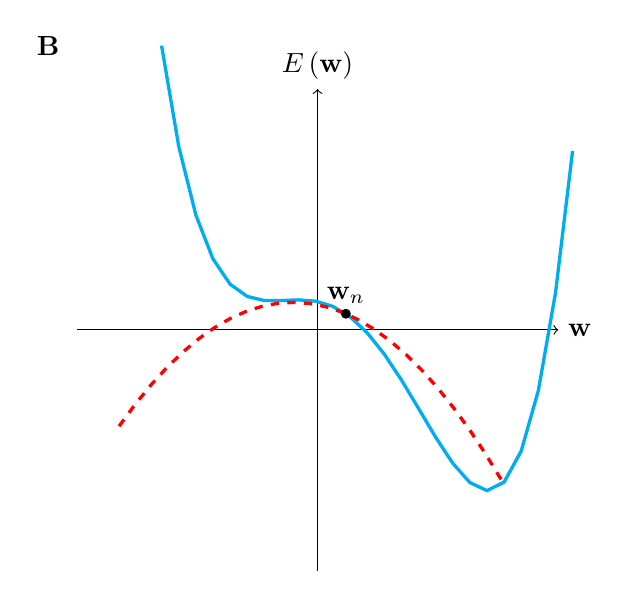
\begin{tikzpicture}[domain=-1.1:1.8,scale=1.8]
%\draw[very thin,color=gray,step=0.25] (-1.4,-1.4) grid (1.4,1.4);
\draw[->] (-1.7,0) -- (1.7,0) node[right]{$\textbf{w}$};
\draw[->] (0,-1.7) -- (0,1.7) node[above]{$E \left( \textbf{w} \right) $};
\draw[very thick,color=cyan] plot (\x,{(\x)^4-(\x)^3-(\x)^2-0.2*\x+0.2});
\draw[very thick,color=red,dashed,domain=-1.4:1.3] plot (\x,{(-1.16/2)*(\x-0.2)^2-0.432*(\x-0.2)+0.1136});
\fill[black,thick]     (0.2,0.1136)    circle (1pt) node [above] {$\textbf{w}_n $}; 
\node[] at (-1.9,2) {\textbf{B}};
\end{tikzpicture}
		\label{fig:aproxlinqw}
	\end{center}	
\end{figure}	
Avaliando o procedimento de aprendizagem de uma rede neural como um problema de otimização, ele passa a ser o equivalente a minimizar a função de erro global, que \'e uma função multivariável  dependente dos pesos da rede .
A maioria dos m\'etodos de minimiza\c{c}\~ao utilizam-se da mesma estrategia .
A minimiza\c{c}\~ao \'e um processo iterativo.
No artigo do M{\o}ller foi desenvolvido uma variação do método do gradiente conjugado que evita executar uma pesquisa linear a cada iteração, utilizando o m\'etodo de Levenberg-Marqurdt \cite{MollerSCG}.
A maioria dos metodos de otimiza\c{c}\~ao utilizam a mesma abordagem, em que a minimiza\c{c}\~ao \'e um algoritmo iterativo onde a cada passo \'e atualizado a dire\c{c}\~ao de busca e a distancia seguindo um algoritmo semelhante \`a de aprendizagem. No SCG ele utiliza-se de uma aproxima\c{c}\~ao da fun\c{c}\~ao erro quadr\'atica ao inv\'ez linear, pois ela consegue convergir de maneira mais rapida como pode-se observar na Figura \ref{fig:aproxlinqw}. Este algoritmo foi implementado para as \ac{ANN} no MATLAB. Um fluxograma constru\'ido a partir da explica\c{c}\~ao do artigo do M{\o}ller est\'a na figura \ref{fig:SCG}.


\begin{figure}[!htp]
	\begin{center}
		\caption{Fluxograma do SCG baseado na explica\c{c}\~ao encontrada no artigo \cite{MollerSCG}}
		\tikzstyle{block} = [
		% The shape:
		rectangle split,
		rectangle split parts =1,
		% The size:
		minimum size=6mm,
		draw,
		text badly centered,
		draw=blue!80!black!40,
		text=black,
	]
\tikzstyle{decision} = [
		diamond,
		draw,
		text badly centered,
		color=blue,
		aspect=2,
		inner sep=1.5pt,
]
\tikzstyle{begin} = [
		rounded rectangle,
		draw,
		text badly centered,
		minimum size = 1cm,
		color=blue,
]
\tikzstyle{coord} = [
-stealth,
inner sep =0 pt,
]
\begin{tikzpicture}[node distance= 0.6cm,
transition/.style={very thick,->}
]

\node [begin] (start) {\textbf{In\'icio}};

\node [block,rectangle split parts=4] (1) [below=of start] 
	 {\nodepart{one} Escolha 
	  \nodepart{two} $\textbf{w}_1$ 
	  \nodepart{three} $0 < \sigma \leq 10^{-4}$
	  \nodepart{four} $0 < \lambda_1  \leq 10^{-6}$
     };

\node [block,rectangle split parts=4] (2) [below=of 1] {
	\nodepart{one} $\textbf{r}_1 = \textbf{r}_1 = E'(\textbf{w}_1) $
	\nodepart{two} $n = 1 $
	\nodepart{three} $ \text{success} = true $
	\nodepart{four} $\overline{\lambda}_1 = 0 $
	};

\node [decision] (3) [below=of 2]{success};

\node [coord] (c1) [right=of 3.east]{};

\node [coord] (c2) [right=of 1.east]{};

\node [block,rectangle split parts = 3] (4) [right=of c2] {
	\nodepart{one} $\sigma _n =\frac{\sigma}{\left| \textbf{p}_n \right| } $
	\nodepart{two} $\textbf{s}_n = \frac{E' ( \textbf{w}_n + \sigma_n \textbf{p}_n) - E' ( \textbf{w}_n )}{ \sigma_n}  $
	\nodepart{three} $\delta_n = \textbf{p}_n \cdot \textbf{s}_n $ 
};

\node [block] (5) [below=of 4] {
	\nodepart{one} $\delta_n =\delta_n + (\lambda_n - \overline{\lambda}_n ) \left| \textbf{p}_n \right| ^2 $
 };

\node [decision] (6) [below=of 5]{ $\delta_n \leq 0 $ };

\node [block,rectangle split parts=3] (7) [below=of 6]{
	\nodepart{one} $ \overline{\lambda}_n = 2 \left( \lambda_n - \frac{\delta_n}{\left| \textbf{p}_n \right| ^2}\right) $ 
	\nodepart{two} $\delta_n = - \delta_n \left| \textbf{p}_n \right| ^2$
	\nodepart{three} $\lambda_n = \overline{\lambda}_n$
};

\node [block, rectangle split parts = 2] (8) [below=of 7]{
	\nodepart{one} $ \mu_n = \textbf{p}_n \cdot \textbf{r}_n $
	\nodepart{two} $ \alpha_n = \frac{\mu_n}{\delta_n}  $
};

\node [block] (9) [below=of 8]{
	\nodepart{one} $\Delta_n = 2 \delta_n \frac{\left[ E(\textbf{w}_n) - E(\textbf{w}_n + \alpha_n \textbf{p}_n) \right]}{\mu_n ^2}$
};

\node [decision] (10) [below=of 9]{
	$\Delta_n \geq 0 $
};


\node [coord] (c3) [right=of 10] {};
\node [coord] (c4) [right=of 4] {};


\node [block,rectangle split parts=4] (11) [right=of c4]{
	\nodepart{one} $\textbf{w}_{n+1} = \textbf{w}_n + \alpha_n \textbf{p}_n$
	\nodepart{two} $\textbf{r}_{n+1} = - E (\textbf{w}_{n+1} )$
	\nodepart{three} $ \overline{\lambda}_n = 0 $
	\nodepart{four} $ success = true $
};

\node [decision] (12) [below=of 11]{$n \text{ mod }N = 0 $};

\node [block](13) [right=of 12]{
	$\textbf{p}_{n+1} = \textbf{r}_{n+1}$
};


\node [coord] (c5) [above=of 11] {};

\node [block, rectangle split parts=2] (14) [below=of 12]{
	\nodepart{one} $\beta_n  =\frac{ \left| \textbf{r}_{n+1}\right|^2 - \textbf{r}_{n} \cdot \textbf{r}_{n+1} }{\mu_n} $
	\nodepart{two} $\textbf{p}_{n+1} = \textbf{r}_{n+1} \beta_n  \textbf{p}_{n} $
};

\node [decision] (15) [below=of 14] {$\Delta_n \geq 0.75 $};

\node [block] (15true) [right=of 15] {$\lambda_n =\frac{1}{4} \lambda_n $};

\node [block,rectangle split parts=2] (16) [below=of 10] {
	\nodepart{one} $\overline{\lambda}_n = \lambda_n $
 	\nodepart{two} $\text{success} = false $
};

\node [decision] (17) [below=of 15] {$ \Delta_n < 0.25$};

\node [block] (17true) [right=of 17] {$\lambda_n = \lambda_n \frac{\delta_k \left( 1- \Delta_n \right) }{\left| \textbf{p}_{n}\right|^2} $ };

\node [decision] (18) [below=of 17] {$ \textbf{r}_n \neq 0 $};

\node [block] (19) [below=of 18] {$ n = n + 1$};

\node [begin] (end) [right=of 19] {\textbf{Fim}};

\node [coord] (c6) [below=of 16]{};

\node [coord] (c7) [left=of 5]{};

%\node [coord] (c8) [right=of 6] {};

\node [coord] (c9) [left=of 7] {};

\draw [transition] (start) -- (1);
\draw [transition] (1) -- (2);
\draw [transition] (2) -- (3);
\draw [transition,color=green] (3.east) -| node [midway,above] {\tiny{\textbf{true}}}  (c1) -| (c2) -- (4.west);
\draw [transition,color=red] (3.south) -| node [midway,below] {\tiny{\textbf{false}}}  (c7) -- (5.west);

\draw [transition] (4) -- (5);
\draw [transition] (5) -- (6);
\draw [transition,color=green] (6) -- node [midway,below,rotate=-90] {\tiny{\textbf{true}}}  (7);
\draw [transition,color=red] (6.west) -| node [midway,above] {\tiny{\textbf{false}}}  (c9) |- (8.west);

\draw [transition] (7) -- (8);
\draw [transition,color=green] (6) -- node [midway,below,rotate=-90] {\tiny{\textbf{true}}}  (7);
\draw [transition] (8) -- (9);
\draw [transition] (9) -- (10);
\draw [transition,color=red] (10) -- node [midway,below,rotate=-90]{\tiny{false}}(16);
\draw [transition,color=green] (10.east) -| node [midway,below] {\textbf{true}}  (c3) -| (c4) |- (11.west);
\draw [transition] (11) -- (12);
\draw [transition,color=green] (12) -- node [midway,below ] {\tiny{\textbf{true}}} (13);
\draw [very thick] (13.north)  edge [ out=90,in = 0,to path={|- (\tikztotarget)}] (c5);
\draw [transition] (c5) -| (4.north);
\draw [transition,color=red] (12) -- node [midway,below,rotate=-90]{\tiny{false}}(14);
\draw [transition] (14) -- (15);
\draw [transition,color=green] (15) -- node [midway,below] {\tiny{\textbf{true}}}  (15true);
\draw [transition,color=red] (15) -- node [midway,below,rotate=-90]{\tiny{false}}(17);
\draw [transition] (15true) |- (17.north);
\draw [transition,color=green] (17) -- node [midway,below] {\tiny{\textbf{true}}}  (17true);
\draw [transition,color=red] (17) -- node [midway,below,rotate=-90]{\tiny{false}}(18);
\draw [transition] (17true) |- (18.north);
\draw [transition,color=red] (18) -- node [midway,below,rotate=-90]{\tiny{false}}(19);
\draw [transition,color=green] (18) -| node [midway,above] {\tiny{\textbf{true}}}  (end);
\draw [transition] (19) |- (c6) -| (3.west);
\end{tikzpicture}
		\label{fig:SCG}
	\end{center}	
\end{figure}

\clearpage
\section{Support Vector Machine(SVM)}
\par
De modo simples as \ac{SVM} são hiperplanos que separam os dados de treinamento para uma margem maxima separando os dados de um lado como -1 e de outro lado o valor 1. As instancias de treinamento que ficam proximas ao hiperplano são chamados de Vetores Suporte. De maneira geral, as \ac{SVM} permitem projetar os dados de treinamento original no espaço X para um espaço F via um kernel K \cite{Haykin2008}.

\ac{SVM} lineares tem sido utilizado com sucesso numa grande variedade de aplica\c{c}\~oes em \ac{BCIs} \cite{RAO}.
Nos casos em que \ac{SVM} linear n\~ao \'e o suficiente, \'e poss\'ivel utilizar-se do \textit{kernel trick} para remapear os dados para um espa\c{c}o dimens\~ao mais alta onde eles s\~ao linearmente separ\'aveis\cite{Vapnik95}\cite{SVM2017}.
\subsection{Hiperplanos}
Na geometria hiperplanos s\~ao um subespa\c{c}o com uma dimens\~ao menor do que o espa\c{c}o no qual ele esta contido. Por exemplo, um hiperplano num plano \'e uma reta. A equa\c{c}\~ao que define um hiperplano \'e eq. \ref{eq:hiperplane}
\begin{equation}\label{eq:hiperplane}
\textbf{w} \cdot \textbf{x} + b = 0
\end{equation}
hiperplanos podem ser utilizados para fazer um classificador bin\'ario se utilizarmos da fun\c{c}\~ao sinal(eq.\ref{eq:sign}) obtemos eq. \ref{eq:linclass} onde os pontos \`a esquerda da reta s\~ao classificados como 1 e os \`a direita como -1 e observe que esse classificador \'e id\^entico a um perceptron de uma camada usando a fun\c{c}\~ao sinal como fun\c{c}\~ao de ativa\c{c}\~ao.
\begin{equation}\label{eq:linclass}
\varphi \left( \textbf{w} \cdot \textbf{x} + b \right) = \textbf{y}
\end{equation}
A desvantagem do perceptron \'e de que ele aleat\'oriamente escolhe um hiperplano detre infinitos poss\'iveis que minimiza o erro (figura \ref{fig:hiperplanos}) \cite{SVM2017}.
\begin{figure}[!htp]
	\begin{center}
		\caption{alguns dos hiperplanos poss\'iveis para a classifica\c{c}\~ao das amostras}
		%\begin{tikzpicture}[&gt;=stealth']
\begin{tikzpicture}
% Draw axes
%\draw [&lt;-&gt;,thick] (0,5) node (yaxis) [above] {$y$}
\draw [thick] (0,5) node (yaxis) [above] {$u$}
|- (5,0) node (xaxis) [right] {$v$};
% draw line
\draw (0,-1) -- (5,4)node[above]{$\textbf{w}_1$}; % y=x-1
\draw (-0.5,1.4) -- (6,1.4)node[above]{$\textbf{w}_2$}; % y=x+1
\draw (3.2,-1) -- (3.2,5) node[above]{$\textbf{w}_3$}; % y=x-3
%\draw[black,<->,very thick]     (1.5,2.5)-- (3.5,0.5) node[above, rotate=-45,midway,xshift=-5]{$D$};% y=-x+4
% \draw labels
%\draw (3.5,3) node[rotate=45,font=\small] 
%{$\mathbf{w}\cdot \mathbf{x} + b = 0$};
%\draw (2.5,4) node[rotate=45,font=\small] 
%{$\mathbf{w}\cdot \mathbf{x} + b = 1$};
%\draw (4.5,2) node[rotate=45,font=\small] 
%{$\mathbf{w}\cdot \mathbf{x} + b = -1$};
% draw distance
%\draw[dotted] (4,5) -- (6,3);
%\draw (5.25,4.25) node[rotate=-45] {$\frac{2}{\Vert \mathbf{w} \Vert}$};
%\draw[dotted] (0,0) -- (0.5,-0.5);
%\draw (0,-0.5) node[rotate=-45] {$\frac{b}{\Vert \mathbf{w} \Vert}$};
%\draw[-&gt;] (2,1) -- (1.5,1.5);
%\draw[thick] (2,1) -- (1.5,1.5);
\draw (1.85,1.35) node[rotate=-45]{}; %{$\mathbf{w}$};
% draw negative dots
\fill[black] (0.5,1.5) circle (3pt);
\fill[black]   (2.5,3.5)   circle (3pt);
\fill[black] (1,2.5)     circle (3pt);
\fill[black] (0.75,2)    circle (3pt);
\fill[black] (0.6,1.9)   circle (3pt);
\fill[black] (0.77, 2.5) circle (3pt);
\fill[black] (1.5,3)     circle (3pt);
\fill[black] (1.3,3.3)   circle (3pt);
\fill[black] (0.6,3.2)   circle (3pt);
% draw positive dots
\draw[black] (4,1)     circle (3pt); 
\draw[black] (3.3,.3)  circle (3pt); 
\draw[black]     (4.5,1.2) circle (3pt); 
\draw[black]     (4.5,.5)  circle (3pt); 
\draw[black]     (3.9,.7)  circle (3pt); 
\draw[black]     (5,1)     circle (3pt); 
\draw[black]     (3.5,.2)  circle (3pt); 
\draw[black]     (4,.3)    circle (3pt); 
\end{tikzpicture}
		\label{fig:hiperplanos}
	\end{center}	
\end{figure}
Isto pode n\~ao parecer problem\'atico at\'e se considerar de que o objetivo do algoritmo n\~ao \'e classificar os dados que n\'os possu\'imos agora mas sim os dados futuros de que ele ir\'a encontrar.
\par
A solu\c{c}\~ao para esse problema foi encontrada por Vapnick  onde ele demonstrou que o hiperplano \'otimo (aquele tem que tem a melhor generaliza\c{c}\~ao) \'e  aquele que criar a maior separa\c{c}\~ao das amostras conhecidas \cite{SVM2017}.
\subsection{Dedu\c{c}\~ao do hiperplano \'otimo}
\begin{figure}[!htp]
	\begin{center}
		\caption{SVM}
		%\begin{tikzpicture}[&gt;=stealth']
\begin{tikzpicture}
% Draw axes
%\draw [&lt;-&gt;,thick] (0,5) node (yaxis) [above] {$y$}
\draw [thick] (0,5) node (yaxis) [above] {$y$}
|- (5,0) node (xaxis) [right] {$x$};
% draw line
\draw (0,-1) -- (5,4); % y=x-1
\draw[dashed] (-1,0) -- (4,5); % y=x+1
\draw[dashed] (2,-1) -- (6,3); % y=x-3
\draw[black,<->,very thick]     (1.5,2.5)-- (3.5,0.5) node[above, rotate=-45,midway,xshift=-5]{$D$};% y=-x+4
% \draw labels
\draw (3.5,3) node[rotate=45,font=\small] 
{$\mathbf{w}\cdot \mathbf{x} + b = 0$};
\draw (2.5,4) node[rotate=45,font=\small] 
{$\mathbf{w}\cdot \mathbf{x} + b = 1$};
\draw (4.5,2) node[rotate=45,font=\small] 
{$\mathbf{w}\cdot \mathbf{x} + b = -1$};
% draw distance
%\draw[dotted] (4,5) -- (6,3);
%\draw (5.25,4.25) node[rotate=-45] {$\frac{2}{\Vert \mathbf{w} \Vert}$};
%\draw[dotted] (0,0) -- (0.5,-0.5);
%\draw (0,-0.5) node[rotate=-45] {$\frac{b}{\Vert \mathbf{w} \Vert}$};
%\draw[-&gt;] (2,1) -- (1.5,1.5);
%\draw[thick] (2,1) -- (1.5,1.5);
\draw (1.85,1.35) node[rotate=-45]{}; %{$\mathbf{w}$};
% draw negative dots
\fill[red] (0.5,1.5) circle (3pt);
\fill[red]   (2.5,3.5)   circle (3pt);
\fill[black] (1,2.5)     circle (3pt);
\fill[black] (0.75,2)    circle (3pt);
\fill[black] (0.6,1.9)   circle (3pt);
\fill[black] (0.77, 2.5) circle (3pt);
\fill[black] (1.5,3)     circle (3pt);
\fill[black] (1.3,3.3)   circle (3pt);
\fill[black] (0.6,3.2)   circle (3pt);
% draw positive dots
\draw[red,thick] (4,1)     circle (3pt); 
\draw[red,thick] (3.3,.3)  circle (3pt); 
\draw[black]     (4.5,1.2) circle (3pt); 
\draw[black]     (4.5,.5)  circle (3pt); 
\draw[black]     (3.9,.7)  circle (3pt); 
\draw[black]     (5,1)     circle (3pt); 
\draw[black]     (3.5,.2)  circle (3pt); 
\draw[black]     (4,.3)    circle (3pt); 
\end{tikzpicture}
		\label{fig:SVM}
	\end{center}	
\end{figure}
Para encontrar o hiperplano \'otimo queremos entrar o hiperplano que maximiza a dist\^ancia $D$ que separa as amostras das duas classes (figura \ref{fig:SVM}). Essa dist\^ancia pode ser obtida atrav\'es da margem geom\'etrica $M$.
\begin{eqnarray}
M = \min_{i=1\dots m} \gamma_i\\
\gamma_i = y_i \frac{\textbf{w}}{\left\| \textbf{w}\right\|} \cdot \textbf{x}_i +{\frac{b}{\left\| \textbf{w} \right\|}}
\end{eqnarray}
onde $y_i$ \'e a classifica\c{c}\~ao do da amostra ($+1$,$-1$) e $x_i$ \'e o vetor de caracter\'isticas da amostra.

Para encontrarmos \textbf{w} e $b$ encontrar a maior margem geom\'etrica \'e equivalente a resolver a equa\c{c}\~ao 
\begin{equation}\label{eq:SVMmin}
\begin{aligned}
& \underset{\textbf{w},b}{\text{minimizar}}
& & \frac{1}{2} {\left\| \textbf{w} \right\|}^{2} \\
& \text{sujeito a}
& & y_i (\textbf{w} \cdot \textbf{x}_i) + b -1 \geq  0, \; i=1,\ldots,m.
\end{aligned}
\end{equation}
Utilizando o m\'etodo de Lagrange que diz que se tiver um problema do tipo
\begin{equation}\label{eq:Lagrange}
\begin{aligned}
& \underset{\textbf{x}}{\text{minimizar}}
& & f\left( \textbf{x} \right)  \\
& \text{sujeito a}
& & y_i (g \left( \textbf{x} \right) = 0.
\end{aligned}
\end{equation}
o minimo de $f\left( \textbf{x} \right)$ \'e encontrado quando o seu gradiente a ponta na mesma dire\c{c}\~ao do gradiente de $g\left( \textbf{x} \right) $ em outras palavras quando
\begin{eqnarray}
\nabla f\left( \textbf{x} \right) = \alpha \nabla g\left( \textbf{x} \right)\\
\nabla f\left( \textbf{x} \right) - \alpha \nabla g\left( \textbf{x} \right)=0\\
\mathcal{L}\left( \textbf{x}, \alpha \right)  = \nabla f\left( \textbf{x} \right) - \alpha \nabla g\left( \textbf{x} \right)
\end{eqnarray}

Utilizando o m\'etodo de Lagrange na equa\c{c}\~ao \ref{eq:SVMmin} obtemos
\begin{equation}\label{eq:SVMLagrange}
\mathcal{L}\left( \textbf{w},b, \alpha \right) =\frac{1}{2} {\left\| \textbf{w} \right\|}^{2} - \sum_{i=1}^{m} \alpha_i \left[ y_i (\textbf{w} \cdot \textbf{x}_i) + b -1 \right] 
\end{equation}
Como o este \'e um problema de minimiza\c{c}\~ao temos as seguintes condi\c{c}\~oes \cite{Haykin2008}:
\begin{equation}\label{eq:SVMLagrangeCD1}
\frac{\partial{\mathcal{L}(\textbf{w},b,\alpha)}}{\partial{\textbf{w}}}=\textbf{0}
\end{equation}
e
\begin{equation}\label{eq:SVMLagrangeCD2}
\frac{\partial{\mathcal{L}(\textbf{w},b,\alpha)}}{\partial{b}}=0
\end{equation}
a partir destas condi\c{c}\~oes podemos obter as seguintes equa\c{c}\~oes:
\begin{eqnarray*}\label{eq:SVMw}
\textbf{w}=\sum_{i=1}^{N}\alpha_i y_i \textbf{x}_i\\
\sum_{i=1}^{N}\alpha_i y_i=0
\end{eqnarray*}
Utilizando o problema dual e simplificando obtemos
\begin{equation}
	\textbf{w}^2= \sum_{i=1}^{N}\sum_{j=1}^{N} \alpha_i \alpha_j y_i y_j \textbf{x}_i \cdot \textbf{x}_j
\end{equation}
E utilizando a fun\c{c}\~ao objetivo $\mathcal{L}(\textbf{w},b,\alpha) = Q(\alpha)$
obtemos a equa\c{c}\~ao final:
\begin{equation}\label{eq:SVMfinal}
	Q(\alpha) = \sum_{i=1}^{N} \alpha_i - \frac{1}{2} \sum_{i=1}^{N} \sum_{j=1}^{N}\alpha_i\alpha_j y_i y_j (\textbf{x}_i \cdot \textbf{x}_j)
\end{equation}

Esta equa\c{c}\~ao pode ser resolvida utilizando m\'etodos de otimiza\c{c}\~ao para problemas convexos.
 Uma explica\c{c}\~ao mais detalhada de como deduzir pode ser encontrada em \cite{SVM2017} e \cite{Haykin2008}.

\subsection{Kernel}
Para dados que n\~ao s\~ao linearmente separaveis \'e possivel fazer o uso do \textit{Kernel Trick}.
O \textit{Kernel Trick} \'e um m\'etodo que consiste em utilizar a propriedade de que para calcular os pesos \'e apenas necessário o produto escalar dos pontos de treinamento \ tal como pode ser visto na equa\c{c}\~ao \ref{eq:SVMfinal}.
Os pontos de treinamento podem ser transformados para um espa\c{c}o vetorial diferente onde eles s\~ao linearmente separáveis.
Um Kernel mapeia o vetor de características para um espa\c{c}o onde os dados s\~ao linearmente separaveis mas onde o produto escalar seja o mesmo.
O Kernel gaussiano \'e um kernel dado pela equa\c{c}\~ao \ref{eq:gausskernel} que mapeia os pontos de treinamento para um espa\c{c}o vetorial com uma dimens\~ao infinita 
\begin{equation}\label{eq:gausskernel}
K_{\text{RBF}}\left( \textbf{x},\textbf{x'} \right) = \text{exp} \left[ -\gamma \left\|  \textbf{x} - \textbf{x'} \right\| \right]  	
\end{equation}
%
%\section{k-Nearest Neighbor (k-NN)}
%O \ac{k-NN} representa um algoritmo de classifica\c{c}\~ao b\'asico, que determina a classse de um ponto de acordo com a classe do ponto mais pr\'oximo.A dist\^ancia entre os pontos pode ser determinada pela \textit{Dist\^ancia Euclidiana}(Eq. \ref{eq:kNNdistance}) \cite{RAO}. 
%Isso pode ser observado na figura \ref{fig:kNN}(A) onde o ponto vazio, cuja classifica\c{c}\~ao inicialmente desconhecida, est\'a mais pr\'oximo dos pontos vermelhos e portanto o algor\'itmo o classificaria como vermelho. A desvantagem deste m\'etodo \'e que ele \'e sens\'ivel a irregularidades nos dados (fig.\ref{fig:kNN}(B)).
%Uma forma de corrigir isso \'e utilizar os $k$ vizinhos pr\'oximos e determinar a classifica\c{c}\~ao como a classe mais comum dentre esses pontos.
%\begin{equation}\label{eq:kNNdistance}
%D(\textbf{x},\textbf{y})= \sqrt{\sum_{n=1}^{N}\left( x_n-y_n\right)}
%\end{equation}x
%
%\begin{figure}[!htp]
%	\begin{center}
%		\caption{NN (A) onde o ponto desconhecido (vazio) \'e classificado como vermelho e (B) onde o ponto desconhecido \'e classificado como preto devido a um ponto preto irregular.}
%		%\begin{tikzpicture}[&gt;=stealth']
\begin{tikzpicture}
% Draw axes
%\draw [&lt;-&gt;,thick] (0,5) node (yaxis) [above] {$y$}
\draw [thick] (0,5) node (yaxis) [above] {$y$}
|- (5,0) node (xaxis) [right] {$x$};
% draw line
% draw negative dots
\fill[black] (0.5,1.2) circle (3pt);
\fill[black]   (1.5,2.3)   circle (3pt);
\fill[black] (1,2.0)     circle (3pt);
\fill[black] (1,1.5)    circle (3pt);
\fill[black] (0.6,1.4)   circle (3pt);
\fill[black] (0.77, 2.2) circle (3pt);
\fill[black] (1.5,3.2)     circle (3pt);
\fill[black] (1.3,2.5)   circle (3pt);
\fill[black] (0.6,3)   circle (3pt);
% draw positive dots
\fill[red] (2,1.2)     circle (3pt); 
\fill[red] (2.3,.5)  circle (3pt); 
\fill[red]     (3.5,1.4) circle (3pt); 
\fill[red]     (3.5,.7)  circle (3pt); 
\fill[red]     (2.9,.9)  circle (3pt); 
\fill[red]     (4,1.2)     circle (3pt); 
\fill[red]     (1.5,.4)  circle (3pt); 
\fill[red]     (2,.5)    circle (3pt);
%draw uknown
\draw[red,thick] (3,1.5) circle(3pt);
\node[-stealth,rectangle] at (-1,5) {\textbf{A}};
\end{tikzpicture}
%		%\begin{tikzpicture}[&gt;=stealth']
%\vspace{50px}
\begin{tikzpicture}
\begin{scope}[shift={(-16.5,-12.1)}]
\scalebox{.5}{

% Draw axes
%\draw [&lt;-&gt;,thick] (0,5) node (yaxis) [above] {$y$}
\draw [thick] (0,5) node (yaxis) [above] {$y$}
|- (5,0) node (xaxis) [right] {$x$};
% draw line
% draw negative dots
\fill[black] (0.5,1.2) circle (3pt);
\fill[black]   (1.5,2.3)   circle (3pt);
\fill[black] (1,2.0)     circle (3pt);
\fill[black] (1,1.5)    circle (3pt);
\fill[black] (0.6,1.4)   circle (3pt);
\fill[black] (0.77, 2.2) circle (3pt);
\fill[black] (1.5,3.2)     circle (3pt);
\fill[black] (1.3,2.5)   circle (3pt);
\fill[black] (0.6,3)   circle (3pt);
\fill[black] (2.5,1.2) circle (3pt);
% draw positive dots
\fill[red] (2,1.2)     circle (3pt); 
\fill[red] (2.3,.5)  circle (3pt); 
\fill[red]     (3.5,1.4) circle (3pt); 
\fill[red]     (3.5,.7)  circle (3pt); 
\fill[red]     (2.9,.9)  circle (3pt); 
\fill[red]     (4,1.2)     circle (3pt); 
\fill[red]     (1.5,.4)  circle (3pt); 
\fill[red]     (2,.5)    circle (3pt);
\fill[red] (2.5,1.7)	circle (3pt);
%draw uknown
\draw[black,thick] (2.8,1.3) circle(3pt);
%\node[-stealth,rectangle] at (-1,5) {\textbf{B}};
}
\end{scope}
\end{tikzpicture}

%		\label{fig:kNN}
%	\end{center}	
%\end{figure}

\section{Avalia\c{c}\~ao de performance de classifica\c{c}\~ao}
%\subsection{Matriz de Confus\~ao}
%A matriz de confus\~ao \'e 
%\begin{figure}[h!]
%	\caption{Matriz de Confu\~ao}
%	\centering
%	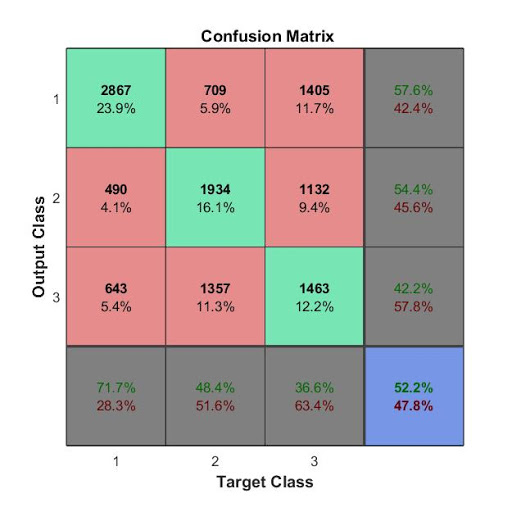
\includegraphics[scale=0.75]{./figuras/confusionmatrix}
%\end{figure}
\subsection{Precis\~ao de classifica\c{c}\~ao}
\par
Precis\~ao de classifica\c{c}\~ao \'e definida como a raz\~ao entre as amostras classificadas corretamente e o numero total de amostras \cite{RAO}.
\begin{equation}\label{eq:ACC}
ACC=\frac{TP+TN}{TP+FN+FP+TN}
\end{equation}
\subsection{Coefficiente Kappa}
Uma outra medida de performance \'e o coeficiente kappa de Cohen:
\begin{equation}\label{eq:kappa}
\kappa=\frac{ACC-ACC_0}{1-ACC_0}
\end{equation}
Onde $ACC$ \'e a precis\~ao de classifica\c{c}\~ao e $ACC_0$ \'e a probabilidade do classificador acertar a classe escolhendo uma classe aleat\'oriamente. Isso torna $\kappa$ uma m\'etrica independente do numero de classes e amostras por classe \cite{RAO}. Um $\kappa = 0$ \'e a performance onde a probabilidade de acerto \'e a mesma que a escolha aleat\'oria e $\kappa = 1$ \'e a performance perfeita.

\clearpage
\section{M\'etodos de estimativa de espectro (PSD)}
\par 
\ac{PSD} extraem informa\c{c}\~oes do sinal como um processo estoc\'astico para descrever a distribui\c{c}\~ao de pot\^encia de um sinal no dom\'inio da frequ\^encia \cite{Comparison2008}.
A \ac{PSD} \'e definido como a transformada de Fourier da fun\c{c}\~ao de autocorrela\c{c}\~ao do sinal contanto que o sinal seja estacion\'ario \cite{Comparison2008}.
Na pr\'atica, as caracter\'isticas estat\'isticas do sinal n\~ao s\~ao conhecidas e s\'o podem ser estimadas de uma sequ\^encia de amostras temporais.
\subsection{Periodograma}
A t\'ecnica de estimativa de espectro $\hat{S}(f)$ mais comum \'e multiplica\c{c}\~ao da transformada de Fourier do sinal $x(t)$ pela sua complexa conjugada, escalonando isto pelo numero de pontos amostrados $N$\cite{PMTM}. 
\begin{equation}
\hat{S}(f)= \frac{X(j2\pi f)  X^{*}(j2\pi f)}{N}
\end{equation}
\begin{equation}\label{eq:winPSD}	
\hat{S}(f)= {\left| \sum_{t=0}^{N-1} x(t) a(t) e^{-2\pi j f t }\right|}^{2} 
\end{equation}
Quando a janela $a(t)$ \'e igual a $1$ ela \'e chamada de janela retangular e esta estimativa \'e chamada de\textbf{ periodograma} \cite{PMTM}.
\par
A confiabilidade da estimativa \'e significativamente reduzida quando h\'a vari\^ancia da estimativa do espectro em cada frequ\^encia $f$ e quando h\'a vazamento de energia em todas frequencias criando um bias\cite{PMTM}.
A vazamento \'e devido ao fato de que utilizamos uma se\c{c}\~ao do sinal que \'e o equivalente a utilizar uma janela retangular.
\cite{PMTM}.
Uma solu\c{c}\~ao a este problema \'e mutiplicar o sinal no dom\'inio do tempo por uma janela n\~ao retangular com uma menor amplitude nas extremidades \cite{PMTM}.
\subsection{Espectro de Welch (PWelch)}
\begin{figure}[!htp]
	\begin{center}
		\caption{Espectro de Welch}
		\scalebox{.8}{
		\tikzstyle{sample}=[minimum height=1cm,minimum width=4cm,xshift=2cm,draw=black]
\tikzstyle{plotsf}=[smooth,yscale=0.05,xscale=8,color=blue]
%\tikzstyle{lines}=[color=black,line width=0.5mm]
\tikzstyle{lines}=[color=black,very thick]
\begin{tikzpicture}[
 brc/.style args = {#1/#2}{decorate,
	decoration={brace, amplitude=5pt,
		raise=#1,#2},% for mirroring of brace
	thick},]
%\begin{axis}[axis line style={draw=none},
%tick style={draw=none},]
%	\addplot table[y=y,x=t,col sep=comma] {./dados/EEG2.csv};
%\end{axis}
\draw (0,0)  [plotsf] plot file {./dados/EEG2.table};
%\draw [thick,double,->] (4.5cm,-3cm)--(4.5cm,-4cm)--(10cm,-4cm) node [midway,below]{\tiny{\textbf{Extra\c{c}\~ao de caracter\'isticas}}};
\draw (0,0) node (s0) [sample,minimum width=16cm,xshift=6cm]{};
\draw [lines, dashdotted ](5.5cm,0.5cm)--(5.5cm,-.5cm);
\draw [lines, dashdotted ](11cm,0.5cm)--(11cm,-0.5cm);
%---------------------------
%Setas para as Janelas FFT
\draw [-latex,very thick](3cm,-0.5cm)--(3cm,-1.8cm)  node[midway,left]{$\hat{S}_1(f)$};
\draw [-latex,very thick](8.5cm,-0.5cm)--(8.5cm,-1.8cm)  node[midway,left]{$\hat{S}_2(f)$};
\draw [-latex,very thick](14cm,-0.5cm)--(14cm,-1.8cm)  node[midway,left]{$\hat{S}_k(f)$};
%---------------------------
%Graficos FFT Janelas
%1
\begin{scope}[xshift=1cm,yshift=-5cm,xscale=-.03,yscale=-.014,rotate=180]%,xcomb]
\draw (-5,0) [color=black,thick]rectangle (125,230);
\draw (0,0)[color=blue,thick]  plot  file {./dados/Welch/W1.table};
\end{scope}
%2
\begin{scope}[xshift=6.5cm,yshift=-5cm,xscale=-.03,yscale=-.014,rotate=180]%,xcomb]
\draw (-5,0) [color=black,thick]rectangle (125,230);
\draw (0,0)[color=blue,thick]  plot  file {./dados/Welch/W2.table};
\end{scope}
%3
\begin{scope}[xshift=12cm,yshift=-5cm,xscale=-.03,yscale=-.014,rotate=180]%,xcomb]
\draw (-5,0) [color=black,thick]rectangle (125,230);
\draw (0,0)[color=blue,thick]  plot  file {./dados/Welch/W3.table};
\end{scope}
%---------------------------
%Espectro de Welch

\begin{scope}[xshift=6.5cm,yshift=-10.5cm,xscale=-.03,yscale=-.014,rotate=180]%,xcomb]
\draw (-5,0) [color=black,thick]rectangle (125,230);
\draw (0,0)[color=blue,thick]  plot  file {./dados/Welch/WMean.table};
\end{scope}
%---------------------------
%SUM
\begin{scope}[xshift=8.3cm,yshift=-6cm]
\node[circle,thick,draw=black] (0,0) {\huge{$+$}};
\end{scope}
%SUM ARROWS
\draw [-latex,very thick](3cm,-5cm)--(3cm,-6cm)--(7.9cm,-6cm);
\draw [-latex,very thick](8.3cm,-5cm)--(8.3cm,-5.5cm);
\draw [-latex,very thick](14cm,-5cm)--(14cm,-6cm)--(8.7cm,-6cm);
%MEAN ARROW
\draw [-latex,very thick](8.3cm,-6.35cm)--(8.3cm,-7.25cm) node[midway,left]{$\frac{1}{K}$};


\end{tikzpicture}
		}
		
		\label{fig:Welch}
	\end{center}	
\end{figure}
O \ac{PWelch}, tamb\'em conhecido como m\'etodo da m\'edia do periodograma consiste em dividir o sinal $x(t)$ em K segmentos $x_k(t)$ parcialmente sobrepostos e calcular a m\'edia do periodograma dos segmentos  \cite{PWelch}.
\begin{equation}
\hat{S}(f)= \frac{1}{K} \sum_{k=1}^{K} \hat{S}_k(f)
\end{equation}
Os passos desse algoritmo podem ser descritos assim:
\pagebreak
\begin{enumerate}
	\item divida o sinal 
	\begin{equation*}
	x[0],x[1],\ldots,X[N-1]
	\end{equation*}
	em $K$ segmentos de comprimento $M$:
	\begin{equation*}
	\begin{aligned}
	\text{Segmento 1: } &x[0],x[1],\ldots,x[M-1]\\
	\text{Segmento 2: } & x[S],x[S+1],\ldots,x[M+S-1]\\
	\vdots & \\
	\text{Segmento K: } & x[N-M],x[N-M+1],\ldots,x[N-1]\\
	\text{onde} &\\
	&M= \text{N\'umero de pontos em cada segmento}\\
	&S= \text{O deslocamento entre os segmentos}\\
	&K = \text{N\'umero de segmentos} \\
	\end{aligned}
	\end{equation*}
	\item Para cada segmento, calcule a \ac{DFT} a uma frequ\^encia $\nu=i/M$:
	\begin{equation*}
	\begin{aligned}
	X_k(\nu)= \sum_m x[m]w[m]e^{-j\pi \ni m}\\
	\text{onde}\\
	m=(k-1)S,\ldots,M+(k-1)S-1\\
	w[m]= a janela\\
	\end{aligned}
	\end{equation*}
	\item Para cada segmento, calcule o valor do periodograma, $P_k(f)$, da transformada de fourier:
	\begin{equation*}
	\begin{aligned}
	P_k(\nu) = \frac{1}{W} {\left| X_k (\nu) \right|}^{2}\\
	onde\\
	W= \sum_{m=0}^{M} w^2 [m]\\  
	\end{aligned}
	\end{equation*}
	\item Calcule a m\'edia dos periodogramas para obter a estimativa de Welch:
	\begin{equation*}
	S_x(\nu)=\frac{1}{K} \sum_{k=1}^{K} P_k(\nu)
	\end{equation*}
\end{enumerate}


\subsection{\textit{Multitaper Power Spectral density} (PMTM)}
\begin{figure}[!htp]
	\begin{center}
		\caption{Multitaper}
		\scalebox{.70}{
		\tikzstyle{sample}=[minimum height=1cm,minimum width=4cm,xshift=2cm,draw=black]
\tikzstyle{plotsf}=[smooth,yscale=0.05,xscale=8,color=blue,]
\tikzstyle{lines}=[color=black,very thick]
\begin{tikzpicture}[
 brc/.style args = {#1/#2}{decorate,
	decoration={brace, amplitude=5pt,
		raise=#1,#2},% for mirroring of brace
	thick},]
	

\begin{scope}[xscale=0.7,yscale=.3]
\begin{axis}[%axis line style={draw=none},
tick style={draw=blue}, yticklabels={,,}, xticklabels={,,},mark repeat=50,ticks=none
]
	\addplot[color=blue] table[y=EEG,x=t,col sep=comma] {./dados/Multitaper/multitaper_all.csv};
\end{axis}
\end{scope}
%----------------------------Tapered EEG--------------
%1
\begin{scope}[xscale=0.7,yscale=.3,yshift=7cm,xshift=8cm]
\begin{axis}[%axis line style={draw=none},
tick style={draw=blue}, yticklabels={,,}, xticklabels={,,},mark repeat=50,ticks=none
]
	\addplot[color=red,loosely dashdotted,very thick] table[y=S1,x=t,col sep=comma] {./dados/Multitaper/multitaper_all.csv};
	\addplot[color=blue] table[y=ES1,x=t,col sep=comma] {./dados/Multitaper/multitaper_all.csv};
\end{axis}
\end{scope}
%2
\begin{scope}[xscale=0.7,yscale=.3,xshift=8cm]
\begin{axis}[%axis line style={draw=none},
tick style={draw=blue}, yticklabels={,,}, xticklabels={,,},mark repeat=50,ticks=none
]
	\addplot[color=red,loosely dashdotted,very thick] table[y=S2,x=t,col sep=comma] {./dados/Multitaper/multitaper_all.csv};
	\addplot[color=blue] table[y=ES2,x=t,col sep=comma] {./dados/Multitaper/multitaper_all.csv};
\end{axis}
\end{scope}
%3
\begin{scope}[xscale=0.7,yscale=.3,yshift=-7cm,xshift=8cm]
\begin{axis}[%axis line style={draw=none},
tick style={draw=blue}, yticklabels={,,}, xticklabels={,,},mark repeat=50,ticks=none
]
	\addplot[color=red,loosely dashdotted,very thick] table[y=S3,x=t,col sep=comma] {./dados/Multitaper/multitaper_all.csv};
	\addplot[color=blue] table[y=ES3,x=t,col sep=comma] {./dados/Multitaper/multitaper_all.csv};
\end{axis}
\end{scope}
%---------------------------Tapered PSDs--------------------
%1
\begin{scope}[xscale=0.55,yscale=.3,yshift=7cm,xshift=21cm]
\begin{axis}[%axis line style={draw=none},
tick style={draw=blue}, yticklabels={,,}, xticklabels={,,},mark repeat=50,ticks=none
]
	\addplot[color=blue] table[y=TS1,x=f,col sep=comma] {./dados/Multitaper/multitaper_all.csv};
\end{axis}
\end{scope}
%2
\begin{scope}[xscale=0.55,yscale=.3,xshift=21cm]
\begin{axis}[%axis line style={draw=none},
tick style={draw=blue}, yticklabels={,,}, xticklabels={,,},mark repeat=50,ticks=none
]
	\addplot[color=blue] table[y=TS2,x=f,col sep=comma] {./dados/Multitaper/multitaper_all.csv};
\end{axis}
\end{scope}
%3
\begin{scope}[xscale=0.55,yscale=.3,yshift=-7cm,xshift=21cm]
\begin{axis}[%axis line style={draw=none},
tick style={draw=blue}, yticklabels={,,}, xticklabels={,,},mark repeat=50,ticks=none
]
	\addplot[color=blue] table[y=TS3,x=f,col sep=comma] {./dados/Multitaper/multitaper_all.csv};
\end{axis}
\end{scope}
%---------------------------------Multitaper---------
\begin{scope}[xscale=0.55,yscale=.3,xshift=32cm]
\begin{axis}[%axis line style={draw=none},
tick style={draw=blue}, yticklabels={,,}, xticklabels={,,},mark repeat=50,ticks=none
]
	\addplot[color=blue] table[y=PSD,x=f,col sep=comma] {./dados/Multitaper/multitaper_all.csv};
\end{axis}
\end{scope}
%-----------------Sum-------------------------
\begin{scope}[xshift=16.5cm,yshift=.8cm]
\node[circle,thick,draw=black] (0,0) {\huge{$+$}};
\end{scope}
%-----------------Arrows----------------------
%-------EEG To Tapered-------
%1
\draw [-latex,very thick](3cm,1.7cm)--(3cm,3cm)--(5.6cm,3cm) node[midway,above]{$\times T_1$};
%2
\draw [-latex,very thick](4.8cm,.8cm)--(5.6cm,.8cm) node[midway,above]{$\times T_2$};
%3
\draw [-latex,very thick](3cm,0cm)--(3cm,-1.4cm)--(5.6cm,-1.4cm) node[midway,above]{$\times T_k$};
%--------Tapered To PSDs------
%1
\draw [-latex,very thick](10.4cm,3cm)--(11.6cm,3cm) node[midway,above]{$\hat{S}_1(f)$};

%2
\draw [-latex,very thick](10.4cm,.8cm)--(11.6cm,.8cm) node[midway,above]{$\hat{S}_2(f)$};

%3
\draw [-latex,very thick](10.4cm,-1.4cm)--(11.6cm,-1.4cm) node[midway,above]{$\hat{S}_k(f)$};
%--------PSDS to Sum-----------
%1
\draw [-latex,very thick](15.3cm,3cm)--(16.5cm,3cm) --(16.5cm,1.2cm) ;

%2
\draw [-latex,very thick](15.3cm,.8cm)--(16.1cm,.8cm) ;

%3
\draw [-latex,very thick](15.3cm,-1.4cm)--(16.5cm,-1.4cm) --(16.5cm,.3cm) ;
%----------Average----------
\draw [-latex,very thick](16.9cm,.8cm)--(17.6cm,.8cm) node[midway,above]{$\frac{1}{K}$};
\end{tikzpicture}
		}

		\label{fig:multitaper}
	\end{center}	
\end{figure}
\par 
\ac{PMTM}, inicialmente descrito por Thomson em 1982, melhora a estimativa espectral ao analisar tanto a vazamento quanto a vari\^ancia na estimativa \cite{PMTM}.
Nesta abordagem, cada janela $v_k$ de um conjunto $K$ de janelas seja ligeiramente diferente e reduza a vazamento de energia em v\'arias frequ\^encias \cite{PMTM}. 
Al\'em disto, as janelas s\~ao ortogonais e s\~ao usadas pra providenciar $K$ amostras ortogonais do sinal $x(t)$.
Estas amostras s\~ao usadas para criar um conjunto de $K$ estimativas $\hat{S}_k (f) $ que podem ser utilizadas para calcular uma  m\'edia $\bar{S}(f)$ com vari\^ancia reduzida \cite{PMTM}.
\begin{equation}
\bar{S}(f) = \frac{1}{K} \sum_{k=1}^{K} \hat{S}_k (f)
\end{equation}
De maneira geral, a aplica\c{c}\~ao de uma janela segue o seguinte padr\~ao: 
Cada janela $a(t)$ \'e associada com uma estimativa de espectro dado pela equa\c{c}\~ao \ref{eq:winPSD} \cite{PMTM}.
Para manter os valores de pot\^encia totais corretos, n\'os assumimos que as janelas s\~ao normalizadas de tal forma que $\sum_{t=0}^{N-1} {\left|  a(t)\right|}^{2}=1 $ \cite{PMTM}. 
Al\'em disso, a pot\^encia do espectro de uma janela $a(t)$ $\left| {A(f)}^{2} \right| $ e suas propriedades s\~ao importantes porque elas determinam, atrav\'es da convolu\c{c}\~ao, a estimativa do nosso espectro do sinal $x(t)$ janelado \cite{PMTM}.
\begin{equation}
\hat{S}(f) = \int_{\frac{-1}{2}}^{\frac{1}{2}} {A(f')}^{2}S(f - f')df'
\end{equation}

\par
Suponha que queremos estimar o nosso espectro com uma banda de resolu\c{c}\~ao $W$, que necessariamente configura um valor entre a resolu\c{c}\~ao do espectro $1/N$ e a frequ\^encia de Nyquist \cite{PMTM}.
Para simplificar a nota\c{c}\~ao assumimos que as amostras entre a unidade e a frequ\^encia de seja normalizado em $\frac{1}{2}$. A fra\c{c}\~ao $\lambda$ da energia da janela dentro da banda selecionada \'e dada por\cite{PMTM}:
\begin{equation}\label{eq:Taper}
\lambda(N,W)=\frac{\int_{-W}^{W}{\left| A(f) \right|}^2 df}{\int_{\frac{1}{2}}^{\frac{1}{2}}{\left| A(f) \right|}^2 df}
\end{equation}

A ideia b\'asicamente \'e de que queremos encontrar as janelas com o m\'inimo de vazamento ao maximizar $\lambda$ a fra\c{c}\~ao de energia dentro da banda $W$ \'e maximizada \cite{PMTM}.
Em suma, $\lambda$ \'e maximizado ao configurar a derivada da express\~ao da equa\c{c}\~ao \ref{eq:Taper} com o vetor $a(t)$ igual a zero \cite{PMTM}.
Isto \'e o equivalente a encontrar os auto valores de uma matriz $N\cross N$ $D$ com os componentes $D_{t,t'}=\frac{2\pi W(t-t')}{\pi(t-t')}$ \cite{PMTM}.
Note de que esta fun\c{c}\~ao \'e sim\'etrica portanto $D$ \'e uma matriz sim\'etrica.
\begin{equation*}
D \cdot \textbf{a} = \lambda \textbf{a}
\end{equation*}
A solu\c{c}\~ao  tem $N$ autovalores $\lambda_k$ e autovetores ($\nu_{1},\nu_{2},\ldots,\nu_{N-1}$) ortonormais  \cite{PMTM}.
O primeiro conjunto de componentes da matriz capturam a maioria das propriedades dessa janela ideal, enquanto os componentes seguintes capturam menos, a quest\~ao \'e quais componentes incluir quando se utiliza eles como janelas\cite{PMTM}. O primeiro autovalor \'e  pr\'oximo de um, portanto ele est\'a associado a um excelente autovetor, em outras palavras uma janela que minimiza o vazamento \cite{PMTM}.